\documentclass{iansnotes}

\title{Use of Binary in Computing}
\author{ian.mcloughlin@atu.ie}
\date{Last updated: \today}

\begin{document}
 
\maketitle

\section{Types}

\begin{minted}{java}
int x = 65;
System.out.println(x);
// 65
System.out.println((char) x);
// A
System.out.println(Integer.toBinaryString(x));
// 1000001
System.out.println((float) x);
// 65.0
int y = Float.floatToIntBits((float) x);
System.out.println(Integer.toBinaryString(y));
// 1000010100000100000000000000000 
\end{minted}

\marcite{oraclefloatingpoint}

\marcite{sanglardfloatingpoint}

\section{Integer Addition}

\begin{tabular}{rrrr}
    & 55 &   &  110111 \\
  + & 33 &   &  100001 \\
  \midrule
    & 88 &   & 1011000 \\
\end{tabular}

\section{Integer Multiply by Two}

\begin{tabular}{rrrrr}
           &  55 & &   &  110111 \\
  $\times$ &   2 & &   &      10 \\
  \midrule
           &     & &   &  000000 \\
  +        &     & &   & 1101110 \\
  \midrule
           & 110 & &   & 1101110 \\
\end{tabular}

\section{Nanometers}
\marcite{ibm2nm}
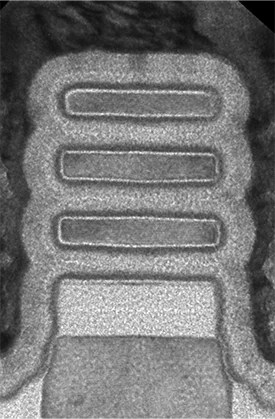
\includegraphics[width=24mm]{img/ibm2nm.png}

\begin{tabular}{rlr}
  \toprule
  nm & Nanometre                & 0.000000001 metres \\
     & Nanometre                &   $10^{-9}$ metres \\
  pm & Picometre                &  $10^{-12}$ metres \\
     & Atomic Radius of Silicon & 111pm              \\
  \bottomrule
\end{tabular}


\section{From Physical to Logical}

\begin{circuitikz}
  \draw
    (4,4) node[npn] {}
    (4,6) node[npn] {}
    (2,4) node[resistorshape] {}
    (2,6) node[resistorshape] {}
    (4,2) node[resistorshape,rotate=90] {}
    (1,4) node[nosshape] {}
    (1,6) node[nosshape] {}
    (0,4) node[vee, rotate=90] {}
    (0,6) node[vee, rotate=90] {}
    (4,7) node[vee] {}
    (4,1) node[ground]{}
    (5,3) node[led,fill=red] {};
\end{circuitikz}
\marcite{circuitdigestandgate}

\end{document} 